\chapter{PJ3}



\section{記分板}

\subsection{次代記分板}
\begin{figure}[h]
  \centering
  \subfigure[次代記分板-1]{
    \includegraphics[width=0.3\textwidth]{timer1.png}
    \label{fig:image1}
  }
  \hfill
  \subfigure[次代記分板-2]{
    \includegraphics[width=0.3\textwidth]{timer2.png}
    \label{fig:image2}
  }
  \hfill
  \subfigure[次代記分板-3]{
    \includegraphics[width=0.3\textwidth]{timer3.png}
    \label{fig:image3}
  }
  \hfill
  \subfigure[次代記分板-4]{
    \includegraphics[width=0.3\textwidth]{timer4.png}
    \label{fig:image3}
  }
  \hfill
  \subfigure[次代記分板-5]{
    \includegraphics[width=0.3\textwidth]{timer1.0-1.png}
    \label{fig:image3}
  }
  \hfill
  \subfigure[次代記分板-6]{
    \includegraphics[width=0.3\textwidth]{timer1.0-3.png}
    \label{fig:image3}
  }
  \hfill
  \subfigure[次代記分板-7]{
    \includegraphics[width=0.3\textwidth]{timer1.0-5.png}
    \label{fig:image3}
  }
  \hfill
  \subfigure[次代記分板-8]{
    \includegraphics[width=0.3\textwidth]{timer1.0-4.png}
    \label{fig:image3}
  }
  \hfill
  \subfigure[次代記分板-9]{
    \includegraphics[width=0.3\textwidth]{timer1.0-2.png}
    \label{fig:image3}
  }
  \caption{次代記分板設計圖}
  \label{fig:multi_images}
\end{figure}


\newpage
\subsection{三代記分板}

\begin{flushleft}
\fontsize{14pt}{20pt}\sectionef\hspace{12pt}\quad 三代的數字都改模成新版的個別分件,通過平面配合各自組裝,使其可更加明顯,且外殼多擴兩孔、齒輪微調和增加輔助軸,使輪盤更方便抓到支點且連動更順滑,雖然變化看起來不大但總體表現都有一定更新
\end{flushleft}

\begin{figure}[h]
  \centering
  \subfigure[三代記分板-1]{
    \includegraphics[width=0.3\textwidth]{timer10.png}
    \label{fig:image1}
  }
  \hfill
  \subfigure[三代記分板-2]{
    \includegraphics[width=0.3\textwidth]{timer9.png}
    \label{fig:image2}
  }
  \hfill
  \subfigure[三代記分板-3]{
    \includegraphics[width=0.3\textwidth]{timer5.png}
    \label{fig:image3}
  }
  \hfill
  \subfigure[三代記分板-4]{
    \includegraphics[width=0.3\textwidth]{timer6.png}
    \label{fig:image3}
  }
  \hfill
  \subfigure[三代記分板-5]{
    \includegraphics[width=0.3\textwidth]{timer2.0-1.png}
    \label{fig:image3}
  }
  \hfill
  \subfigure[三代記分板-6]{
    \includegraphics[width=0.3\textwidth]{timer2.0-3.png}
    \label{fig:image3}
  }
  \hfill
  \subfigure[三代記分板-7]{
    \includegraphics[width=0.3\textwidth]{timer2.0-5.png}
    \label{fig:image3}
  }
  \hfill
  \subfigure[三代記分板-8]{
    \includegraphics[width=0.3\textwidth]{timer2.0-4.png}
    \label{fig:image3}
  }
  \hfill
  \subfigure[三代記分板-9]{
    \includegraphics[width=0.3\textwidth]{timer2.0-2.png}
    \label{fig:image3}
  }
  \caption{三代記分板設計圖}
  \label{fig:multi_images}
\end{figure}


\begin{flushleft}
\fontsize{14pt}{20pt}\sectionef\hspace{12pt}\quad 更新記分板外殼,因舊版顯示方式不清楚。
\end{flushleft}

\begin{figure}[h]
  \centering
  \subfigure[改良三代記分板-1]{
    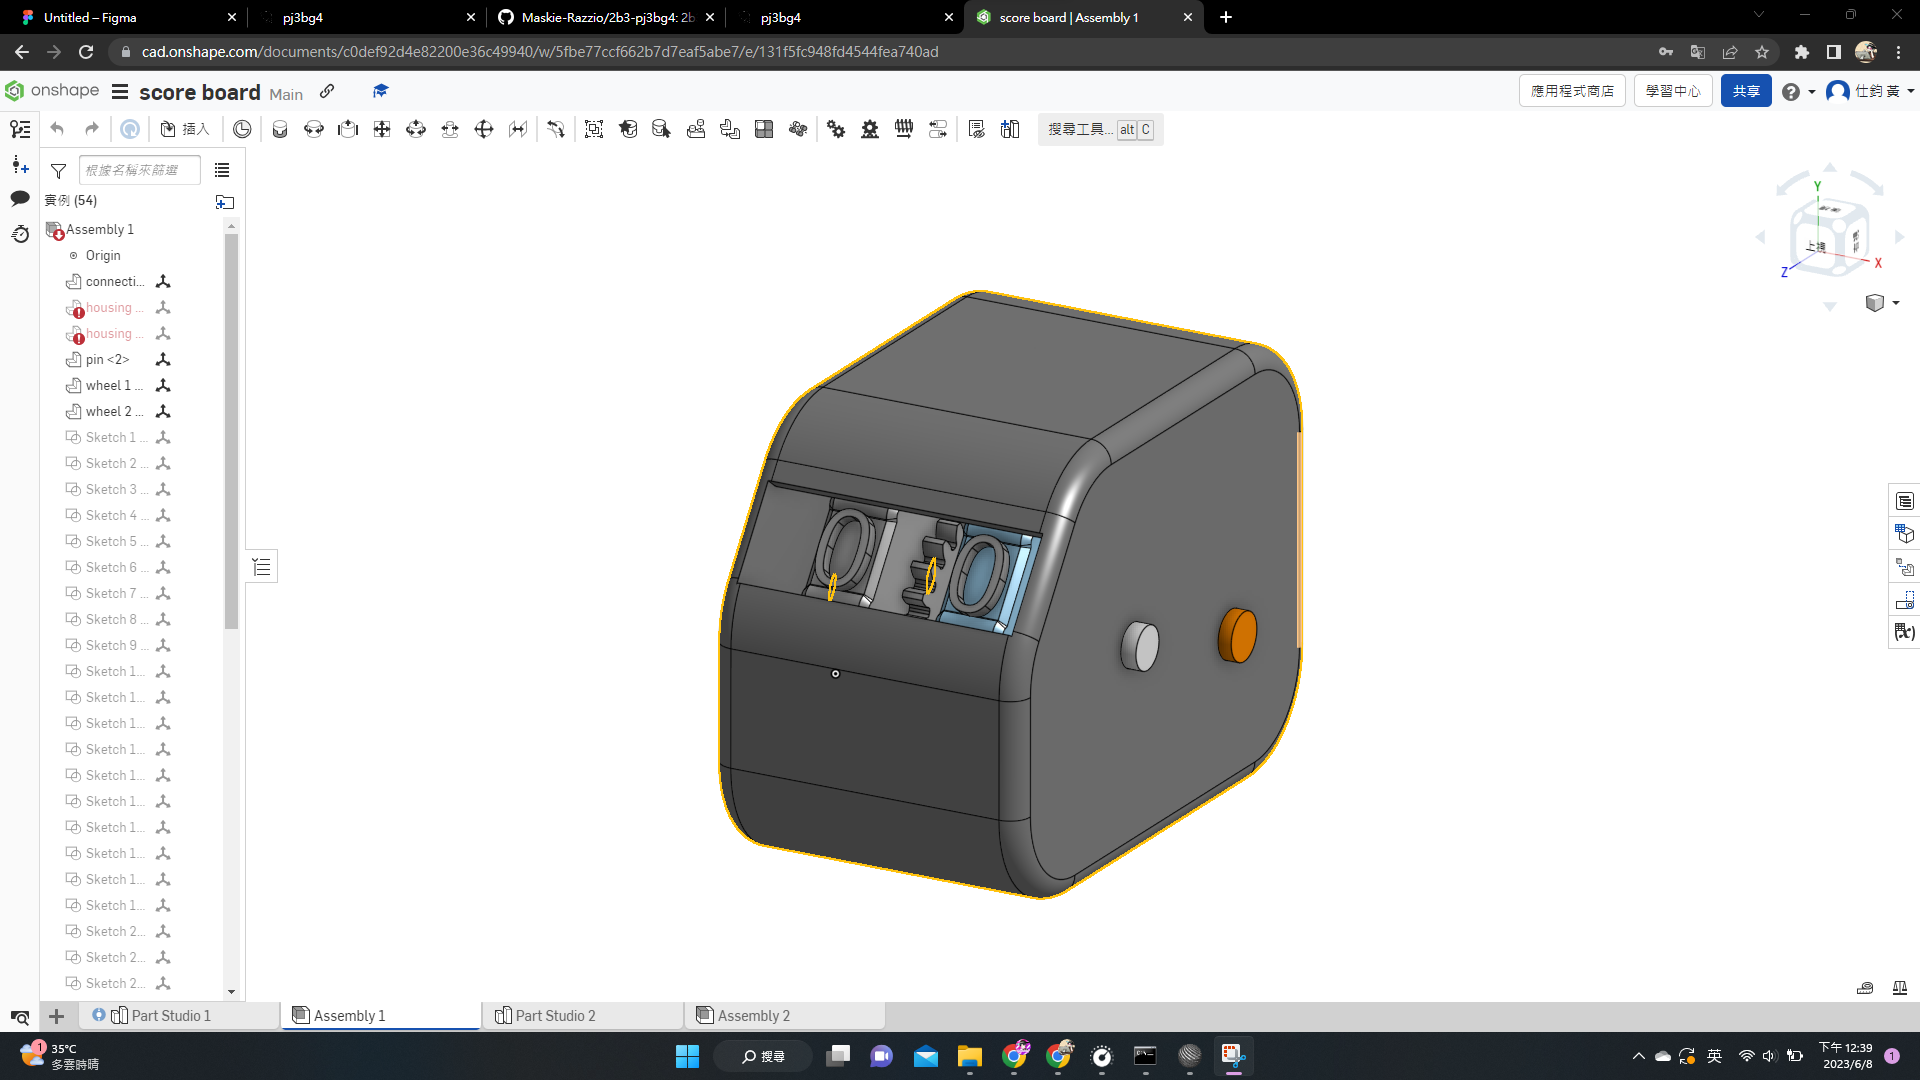
\includegraphics[width=0.3\textwidth]{螢幕擷取畫面 2023-06-08 123921.png}
    \label{fig:image1}
  }
  \hfill
  \subfigure[改良三代記分板-2]{
    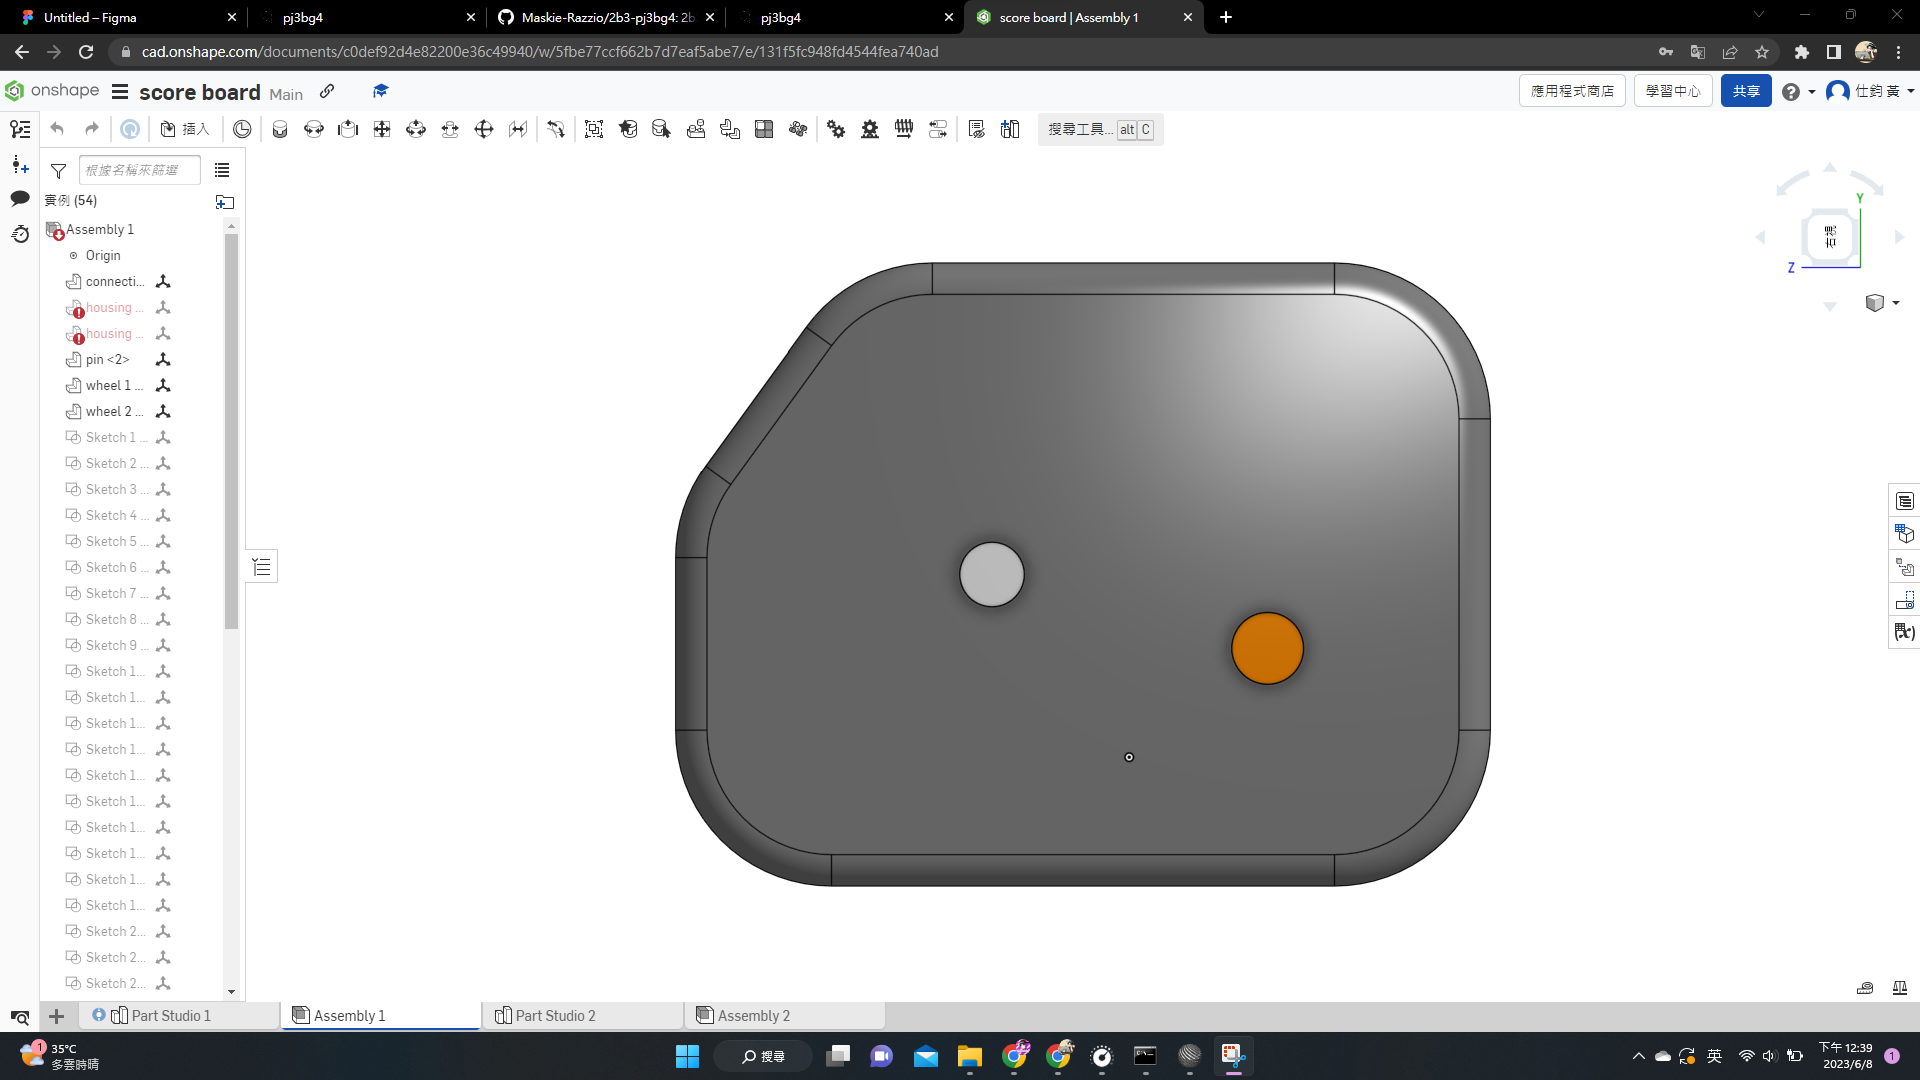
\includegraphics[width=0.3\textwidth]{螢幕擷取畫面 2023-06-08 124004.png}
    \label{fig:image2}
  }
  \hfill
  \subfigure[改良三代記分板-3]{
    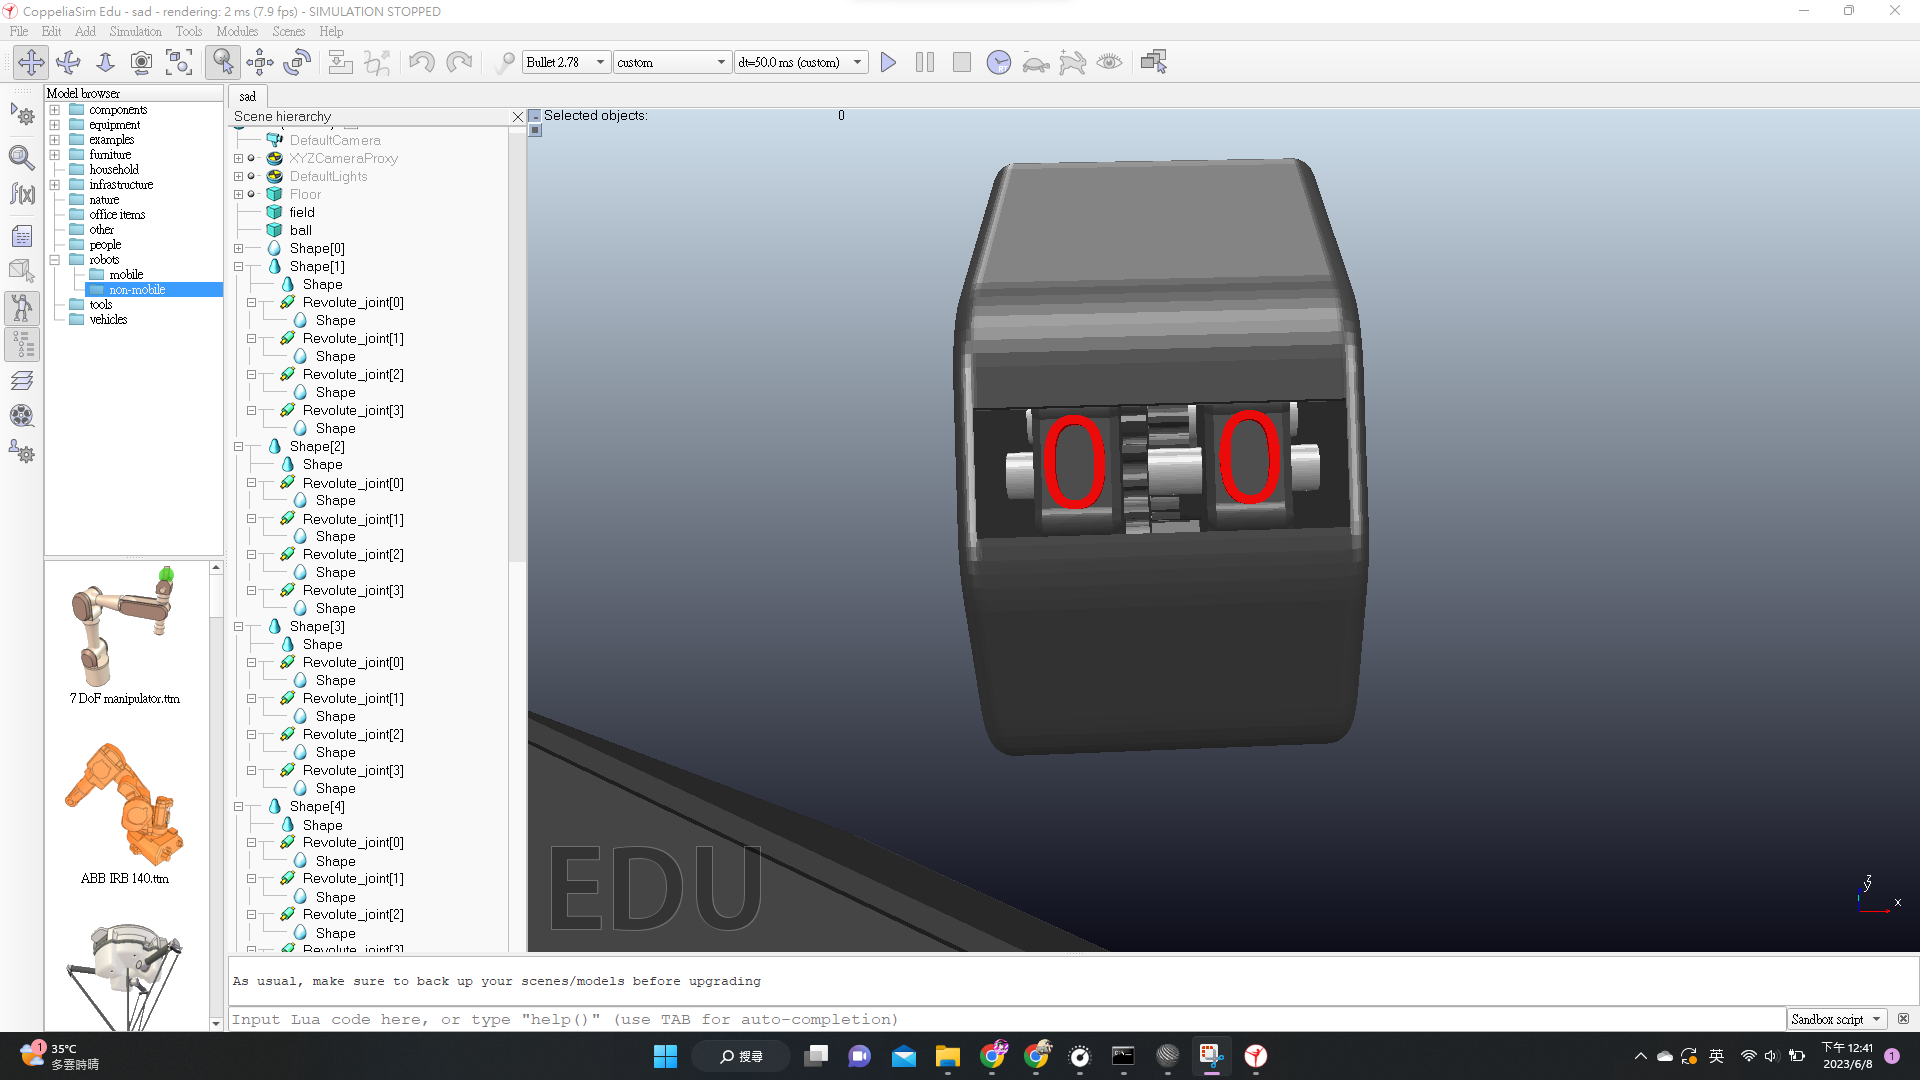
\includegraphics[width=0.3\textwidth]{螢幕擷取畫面 2023-06-08 124125.png}
    \label{fig:image3}
  }
  \hfill

  \caption{改良三代記分板設計圖}
  \label{fig:multi_images}
\end{figure}






\newpage
\section{球員}

\subsection{666系列:}
\begin{figure}[h]
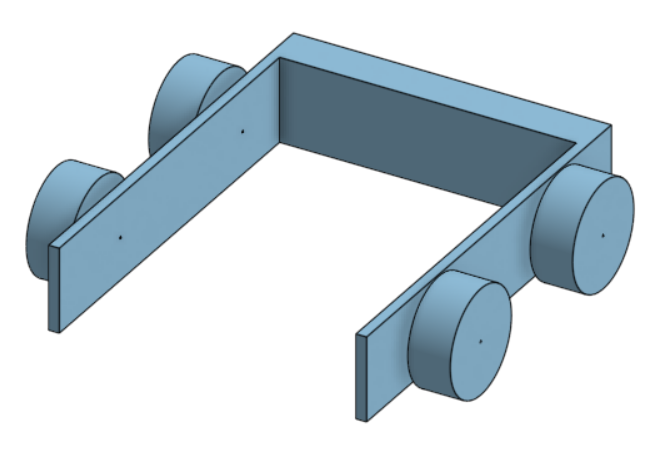
\includegraphics[width=0.5\textwidth]{666.png}
\caption{41023228測試用666}
\end{figure}

\subsection{robot-00系列:}
\begin{figure}[h]
\includegraphics[width=0.5\textwidth]{robot-00系列.png}
\caption{由41023247製作}
\end{figure}

\newpage
\subsection{Maskie Razzio系列:}

\begin{figure}[h]
  \centering
  \subfigure[機器人2:bulldozer6]{
    \includegraphics[width=0.3\textwidth]{bulldozer6.png}
    \label{fig:image1}
  }
  \hfill
  \subfigure[機器人3:bulldozer4]{
    \includegraphics[width=0.3\textwidth]{bulldozer4.png}
    \label{fig:image2}
  }
  \hfill
  \subfigure[機器人4:tank]{
    \includegraphics[width=0.3\textwidth]{tank.png}
    \label{fig:image3}
  }
  \hfill
  \subfigure[機器人5:castle]{
    \includegraphics[width=0.3\textwidth]{castle.png}
    \label{fig:image3}
  }
  \hfill
  \subfigure[機器人6:Eye of Sauron]{
    \includegraphics[width=0.3\textwidth]{eye.png}
    \label{fig:image3}
  }
  \hfill
  \subfigure[機器人7:cat]{
    \includegraphics[width=0.3\textwidth]{cat.png}
    \label{fig:image3}
  }
  \hfill
  \subfigure[機器人8:battlebot]{
    \includegraphics[width=0.3\textwidth]{battlebot.png}
    \label{fig:image3}
  }
  \hfill
  \subfigure[機器人?:wheelchair]{
    \includegraphics[width=0.3\textwidth]{wheelchair.png}
    \label{fig:image3}
  }
  \hfill
  
  \caption{Maskie Razzio系列}
  \label{fig:multi_images}
\end{figure}

\newpage
\subsection{四代與五代球員}

\begin{flushleft}
\fontsize{14pt}{20pt}\sectionef\hspace{12pt}\quad 由於將前幾代球員放入CoppeliaSim裡,會使CoppeliaSim之幀數過高,使其整體運行過慢,因此將機器人重新設計。
\end{flushleft}

\begin{figure}[h]
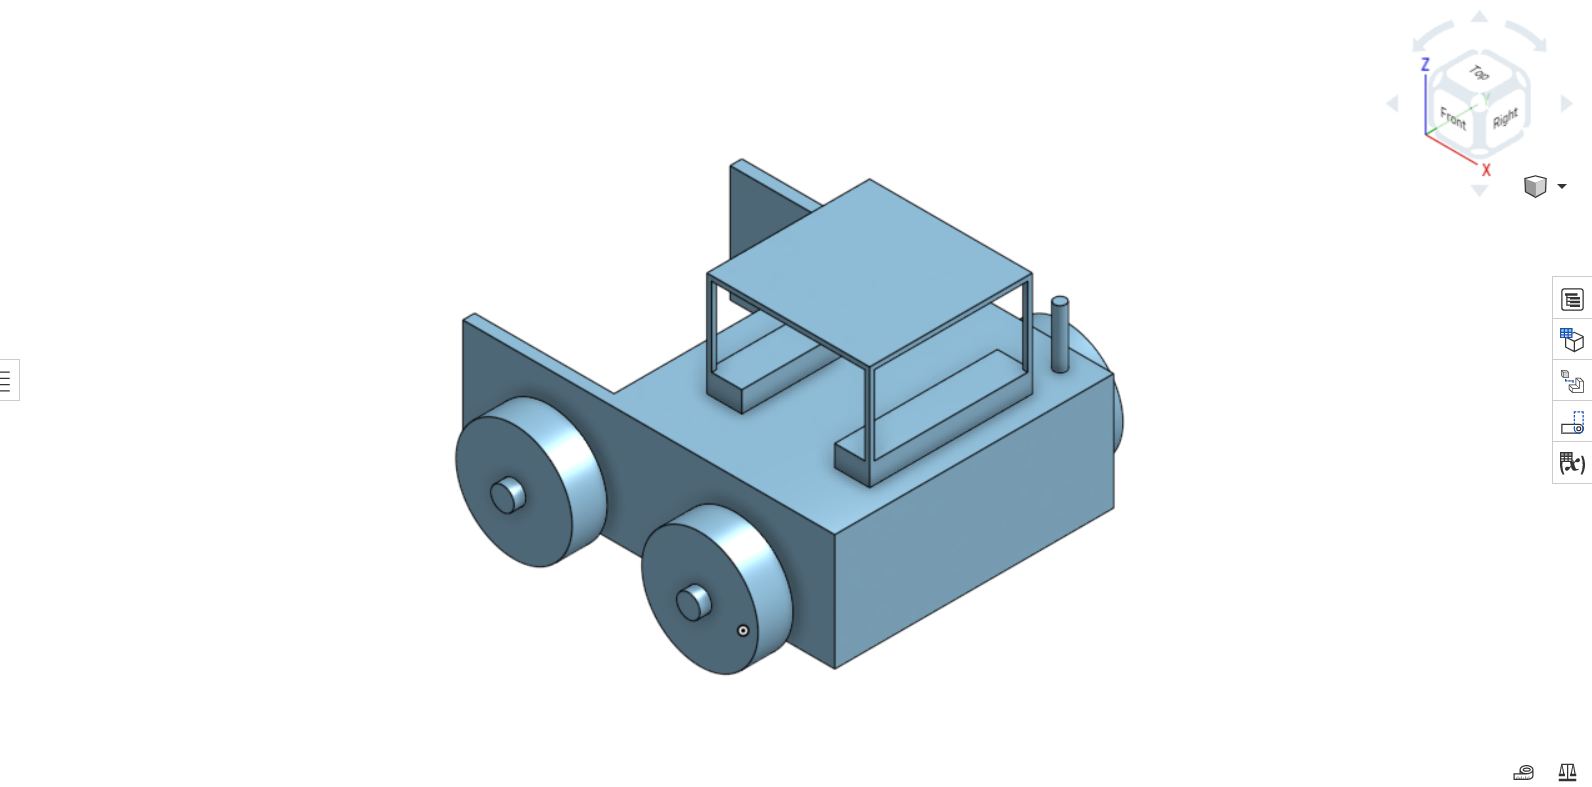
\includegraphics[width=0.5\textwidth]{robot-cccccc系列.png}
\caption{四代球員:robot-cccccc系列}
\end{figure}

\begin{figure}[h]
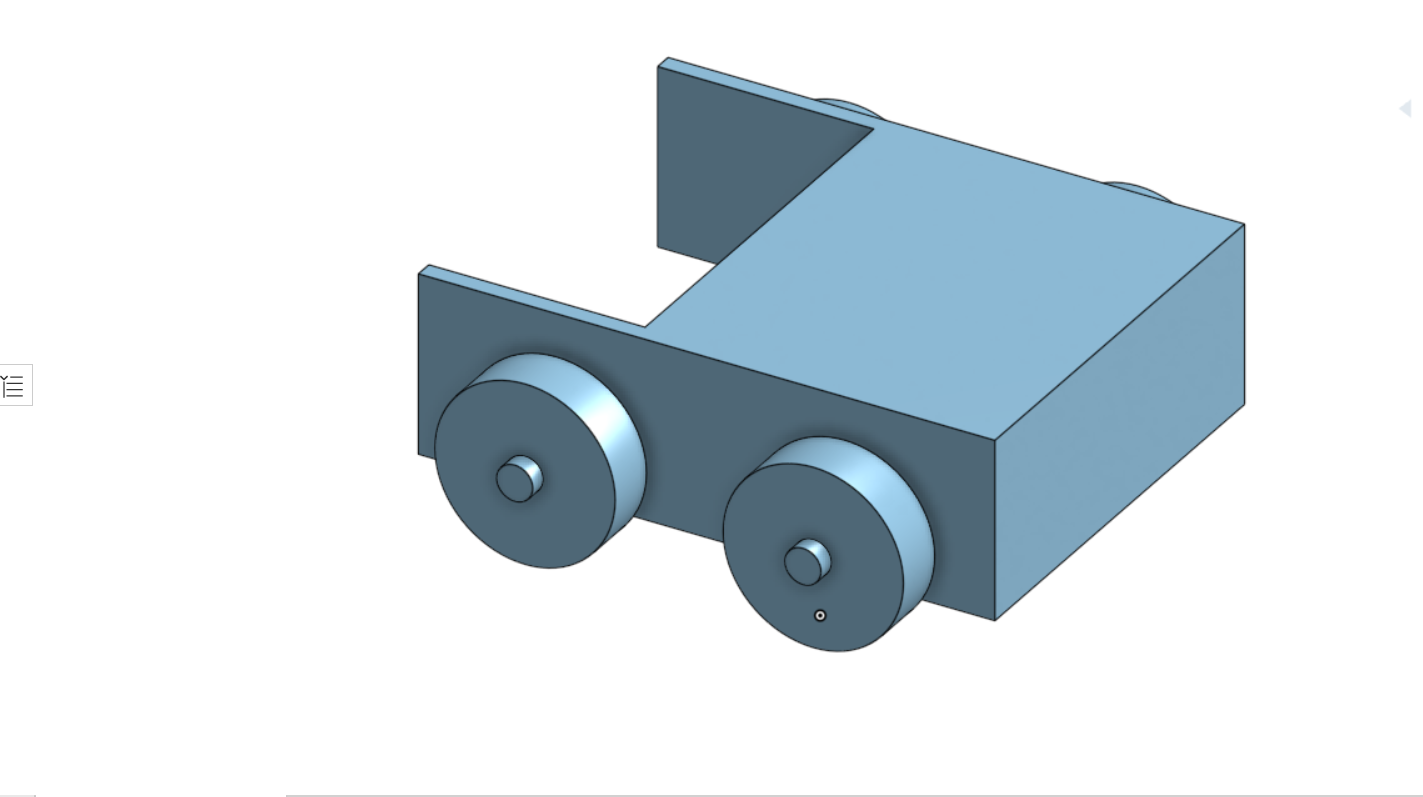
\includegraphics[width=0.5\textwidth]{robot-110系列.png}
\caption{五代球員:robot-110系列}
\end{figure}